% to change the appearance of the header, questions, problems or subproblems, see the homework.cls file or
% override the \Problem, \Subproblem, \question or \printtitle commands.

% The hidequestions option hides the questions. Remove it to print the questions in the text.

\title{MAC4722 - Lista 6}

\documentclass{homework}

\usepackage[utf8]{inputenc}
\usepackage{amsthm}
\usepackage{mathtools}

\usepackage{tikz}
\usetikzlibrary{automata,positioning}

\usepackage{graphicx}
\graphicspath{ {images/} }

\newtheorem*{theorem}{Forma Normal de Chomsky}

% Set up your name, the course name and the homework set number.
\homeworksetup{
    username={Jean Fobe, N$^o$USP 7630573},
    course={Linguagens, Autômatos e Computabilidade - MAC4722},
    setnumber=6}
\begin{document}% this also prints the header.
\pagestyle{fancy}
\fancyfoot[L]{Jean Fobe, 7630573}

% use starred problems or subproblems to apply manual numbering.
\problem*{2}
\question{Escreva uma gramática livre de contexto para cada uma das linguagens a seguir. Explique cada uma das regras de substituição de sua gramática para justificar porque a linguagem gerada pela sua gramática é a correspondente linguagem do enunciado.}
	\begin{itemize}
		\item[(b)] O complemento da linguagem $\{a^n b^n:\ n \geq 0\}$\\
		$Resp:$ Antes de escrever uma gramática vamos antes explicitar o complemento da linguagem acima nos seguintes casos (Admitimos aqui que $\Sigma = \{a,b\}$):
		\begin{enumerate}
			\item $\{a^n b^m:\ n,m \geq 0\ e\ n \neq m\}$;
			\item $\{b x:\ x \in \{a,b\}^*\}$;
			\item $\{a^n b^n y:\ n \geq 0,\ y \in \{a,b\}^+\}$;
		\end{enumerate}		 Existe uma gramática $G = (V, \Sigma, R, S)$ que gera o complemento de $\{a^n b^n:\ n \geq 0\}$, onde: % ($https://math.stackexchange.com/questions/550756/how-to-create-a-grammar-for-complement-of-anbn$)
		\begin{align*}
			V &= \{S, A, B, C, I\};\\
			\Sigma &= \{a,b\};\\
			R &= \{S \rightarrow AI\ |\ IB\ |\ bC\ |\ AIBC,\\
			(1^o\ caso)\ A & \rightarrow aA\ |\ a,\\
			(1^o\ caso)\ B & \rightarrow Bb\ |\ b,\\
			(2^o\ caso)\ C & \rightarrow Ca\ |\ Cb\ |\ \lambda,\\
			(3^o\ caso)\ I & \rightarrow AIB\ |\ \lambda\};
		\end{align*}
		Observando as palavras que as regras geram:
		\begin{align*}
			\forall w \in \Sigma^*,\  AI & \xRightarrow[\text{G}]{*} w \iff w = a^i b^j,\ i > j\geq 0;\\
			\forall w \in \Sigma^*,\  IB & \xRightarrow[\text{G}]{*} w \iff w = a^i b^j,\ j > i \geq 0;\\
			\forall w \in \Sigma^*,\  C & \xRightarrow[\text{G}]{*} w \iff w \in \Sigma^*;\\
			\forall w \in \Sigma^*,\  AIBC & \xRightarrow[\text{G}]{*} w \iff wy,\ w = a^m b^n,\ m,n \geq 0,\ y \in \Sigma^*;
		\end{align*}
		Dessa forma justificamos que $G$ gera a linguagem acima.

\newpage		
		
		\item[(c)] $\{a^m b^n c^p d^q:\ m,n,p,q \geq 0\ e\ m + n = p + q\}$\\
		$Resp:$ Extraímos da descrição acima que $|a^m b^n| = |c^p d^q|$, então uma gramática $G = (V, \Sigma, R, S)$ para gerar essa linguagem pode ser dada da seguinte forma: % $(https://cs.stackexchange.com/questions/83150/is-this-language-context-free-l-ambncpdq-mn-pq)$
		\begin{align*}
			V &= \{S, A, B, C, D\};\\
			\Sigma &= \{a,b,c,d\};\\
			R &= \{S \rightarrow ABD,\\
				&\qquad	A \rightarrow aA\ |\ \lambda, \\
				&\qquad	B \rightarrow bCc\ |\ ABD\ |\ \lambda, \\
				&\qquad	C \rightarrow bC\ |\ Cc\ |\ \lambda, \\
				&\qquad	D \rightarrow Dd\ |\ \lambda\};
		\end{align*}
		Agora observemos as palavras que as regras geram:
		\begin{align*}
			\forall w \in \Sigma^*,\  A & \xRightarrow[\text{G}]{*} w \iff w = a^i,\ i \geq 0;\\
			\forall w \in \Sigma^*,\  D & \xRightarrow[\text{G}]{*} w \iff w = d^i,\ i \geq 0;\\
			\forall w \in \Sigma^*,\  C & \xRightarrow[\text{G}]{*} w \iff w = b^i c^j,\ i,j \geq 0;\\
			\forall w \in \Sigma^*,\ ABD  & \xRightarrow[\text{G}]{*} w \iff w = a^m b^n c^p d^q,\ m,n,p,q \geq 0;
		\end{align*}
		Admitindo não-determinismo, conseguimos gerar todas as palavras da linguagem a partir de $G$, com prefixo de 'a's e 'b's de igual tamanho ao sufixo de 'c's e 'd's, $|a^m b^n| = |c^p d^q|,\ m,n,p,q \geq 0$.
	\end{itemize}
\pagebreak

\problem*{3}
\question{Mostre que se G é uma gramática livre de contexto na Forma Normal de Chomsky então, para cada palavra não vazia $w \in L(G)$ são necessários exatamente $2|w| - 1$ passos em qualquer derivação de w.}
	\begin{theorem}
		(Sipser p. 107, definição 2.8) Uma gramática livre de contexto está na \textbf{forma normal de Chomsky} se todas as suas regras são dadas na forma:
		\begin{align*}
			A & \rightarrow BC; \\
			A & \rightarrow a;
		\end{align*}
		Onde $a$ is any terminal e $A,B,C$ são variáveis quaisqueres, com $B$ ou $C$ não sendo variável de início. Adicionalmente, é permitida a regra $S \rightarrow \lambda$, em que $S$ é a variável inicial.  
	\end{theorem}
	$Resp:$ Seja $|w| = n, n \geq 1$. Podemos derivar a palavra $w$ a partir de uma gramática $G$ na \textbf{forma normal de Chomsky}. A derivação inicia pela variável $S$, com $|S| = 1$.
		\begin{itemize}
			\item Usando $n-1$ regras da forma $A \rightarrow BC\ (variavel \rightarrow variavel\ variavel)$, construímos uma palavra formada por apenas variáveis de tamanho $n$.
			\item Podemos, então, aplicar a regra do tipo $A \rightarrow a\ (variavel \rightarrow simbolo)$ na palavra de tamanho $n$, realizando mais $n$ derivações e chegando na palavra $w$.
			\item  No total aplicamos $(n - 1) + n = 2n -1$ passos de derivação para chegar em $w$. Em expressões:
		\end{itemize}

		\begin{align}
			& |w| = n,\ n \geq 1; \\			
			& S \xRightarrow[\text{G}]{} V_1V_2\ \xRightarrow[\text{G}]{n-2} V_1V_2...V_n,\  (V_1,V_2,...,V_n\ todas\ variaveis\ de\ G); \\
			& V_1V_2...V_n \xRightarrow[\text{G}]{n} w;\\
			& S \xRightarrow[\text{G}]{2n - 1} w
		\end{align}
		
\newpage

\problem*{4}
\question{Construa autômatos com pilha (sem utilizar gramática) que reconheçam as linguagens de alguns dos exercícios anteriores (especificados a seguir). Explique detalhadamente a sua construção. Obs.: Exiba o diagrama de estados e descreva também
todos os componentes da definição formal.}
	\begin{itemize}
		\item[2.a)] ($L = \{a^i b^{2i}: i \geq 0\}$) Seja um automato finito não determinístico $M = (Q, \Sigma, \Gamma, \delta, q_0, F)$, tal que $L(M) = L$,
		\begin{align*}
			Q & = \{q_0,q_1,q_2,q_3,q_f\},\\
			\Sigma & = \{a,b\},\\
			\Gamma & = \{A,\#\},\\
			F & = \{q_f\},\\
			\delta & : Q \times \Sigma \times \Gamma_\lambda \rightarrow P(Q \times \Gamma_\lambda),\ dada\ por:\\
			\delta & (q_0, a, \lambda) = \{(q_1,\#)\};\\
			\delta & (q_1, a, \lambda) = \{(q_2,A)\};\\
			\delta & (q_1, b, A) = \{(q_3,\lambda)\};\\
			\delta & (q_2, \lambda, \lambda) = \{(q_1,A)\};\\
			\delta & (q_3, b, A) = \{(q_3,\lambda)\};\\
			\delta & (q_3, b, \#) = \{(q_f,\lambda)\};\\			
			\delta & (q_f, \lambda, \#) = \{(q_f,\lambda)\} \ (para\ outras\ triplas\ \delta = \emptyset).			
		\end{align*}
		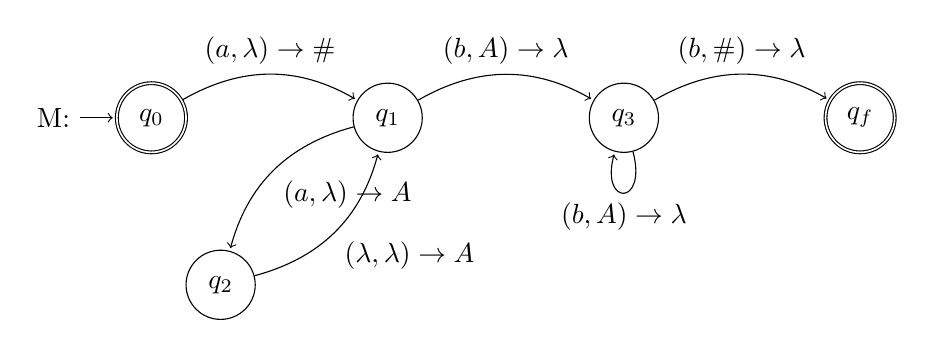
\begin{tikzpicture}[shorten >=1pt,node distance=3cm,on grid,auto,initial text=M:] 
    	\node[state,initial,accepting] (q_0)   {$q_0$}; 
    	\node[state] (q_1) [right=of q_0] {$q_1$}; 
  		\node[state] (q_2) [below left=of q_1] {$q_2$};
    	\node[state] (q_3) [right=of q_1] {$q_3$};
    	\node[state,accepting] (q_f) [right=of q_3] {$q_f$};
        \path[->] 
        (q_0) edge [bend left] node {$(a,\lambda) \rightarrow \#$} (q_1)
        (q_1) edge [bend right] node {$(a,\lambda) \rightarrow A$} (q_2)
        	  edge [bend left] node {$(b,A) \rightarrow \lambda$} (q_3)
        (q_2) edge [bend right] node [swap] {$(\lambda,\lambda) \rightarrow A$} (q_1)
        (q_3) edge [bend left] node {$(b,\#) \rightarrow \lambda$} (q_f)
        	  edge [loop below] node {$(b,A) \rightarrow \lambda$} ()
              ;
	\end{tikzpicture}
	
\newpage	
	
		\item[2.b)] ($L = \overline{\{a^n, b^n: n \geq 0\}}$) Seja um automato finito não determinístico $M = (Q, \Sigma, \Gamma, \delta, q_0, F)$, tal que $L(M) = L$,
		\begin{align*}
			Q & = \{q_0,q_1,q_2,q_3,q_f\},\\
			\Sigma & = \{a,b\},\\
			\Gamma & = \{A,\#\},\\
			F & = \{q_f\},\\
			\delta & : Q \times \Sigma \times \Gamma_\lambda \rightarrow P(Q \times \Gamma_\lambda),\ dada\ por:\\
			\delta & (q_0, a, \lambda) = \{(q_1,\#)\};\\
			\delta & (q_0, b, \lambda) = \{(q_f,\lambda)\};\\
			\delta & (q_1, a, \lambda) = \{(q_1,A)\};\\
			\delta & (q_1, b, \#) = \{(q_2,\lambda)\};\\
			\delta & (q_1, b, A) = \{(q_2,\lambda)\};\\
			\delta & (q_2, a, \lambda) = \{(q_f,\lambda)\};\\
			\delta & (q_2, b, A) = \{(q_2,\lambda)\};\\
			\delta & (q_2, b, \#) = \{(q_3,\lambda)\};\\
			\delta & (q_3, a, \lambda) = \{(q_f,\lambda)\};\\
			\delta & (q_3, b, \lambda) = \{(q_f,\lambda)\};\\
			\delta & (q_f, \lambda, \#) = \{(q_f,\lambda)\};\\
			\delta & (q_f, \lambda, A) = \{(q_f,\lambda)\} \ (para\ outras\ triplas\ \delta = \emptyset).
		\end{align*}
		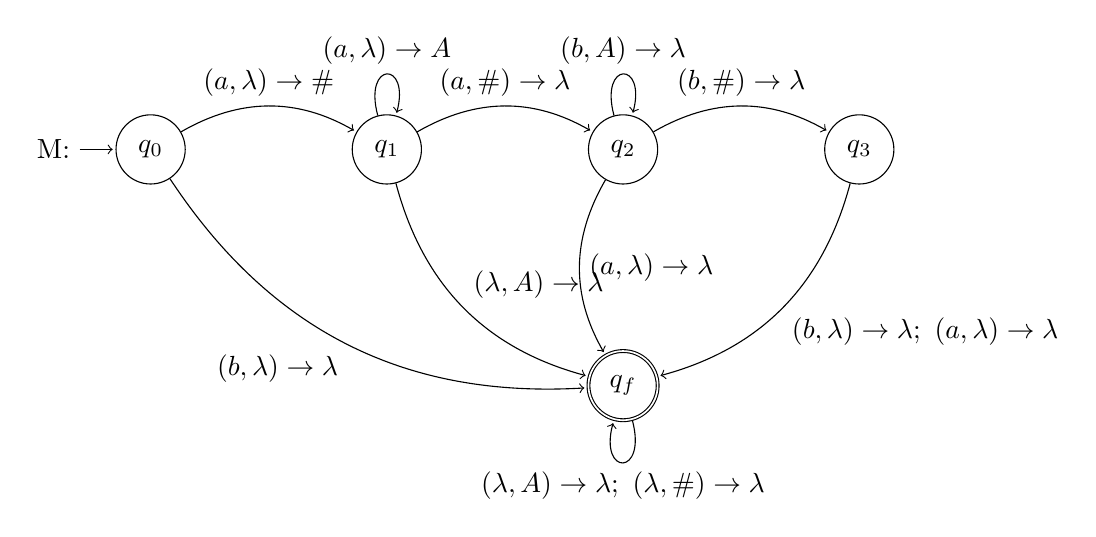
\begin{tikzpicture}[shorten >=1pt,node distance=3cm,on grid,auto,initial text=M:] 
    	\node[state,initial] (q_0)   {$q_0$}; 
    	\node[state] (q_1) [right=of q_0] {$q_1$}; 
  		\node[state] (q_2) [right=of q_1] {$q_2$};
    	\node[state] (q_3) [right=of q_2] {$q_3$};
    	\node[state,accepting] (q_f) [below=of q_2] {$q_f$};
        \path[->] 
        (q_0) edge [bend right] node [swap] {$(b,\lambda) \rightarrow \lambda$} (q_f)
              edge [bend left] node {$(a,\lambda) \rightarrow \#$} (q_1)
        (q_1) edge [bend left] node {$(a,\#) \rightarrow \lambda$} (q_2)
        	  edge [bend right] node {$(\lambda,A) \rightarrow \lambda$} (q_f)
        	  edge [loop above] node {$(a,\lambda) \rightarrow A$} ()
        (q_2) edge [bend right] node {$(a,\lambda) \rightarrow \lambda$} (q_f)
        	  edge [bend left] node {$(b,\#) \rightarrow \lambda$} (q_3)
          	  edge [loop above] node {$(b,A) \rightarrow \lambda$} ()
        (q_3) edge [bend left] node {$(b,\lambda) \rightarrow \lambda;\\$
        							 $(a,\lambda) \rightarrow \lambda$} (q_f)
        (q_f) edge [loop below] node {$(\lambda,A) \rightarrow \lambda;\\$
        							  $(\lambda,\#) \rightarrow \lambda$} ()
              ;
	\end{tikzpicture}
	\end{itemize}
\end{document}
